\documentclass{article}
\usepackage{subcaption}
\usepackage[labelformat=parens,labelsep=quad, skip=3pt]{caption}
\usepackage{graphicx}
\usepackage[font=small,labelfont=bf]{caption}
\usepackage{geometry}

\geometry{
 a4paper,
 left=0mm,
 top=0mm,
 }

\begin{document}


\begin{figure}[htp]
 \centering
\begin{subfigure}{.33\textwidth}
 \caption{Atlantic dFe - cGEnIE}
 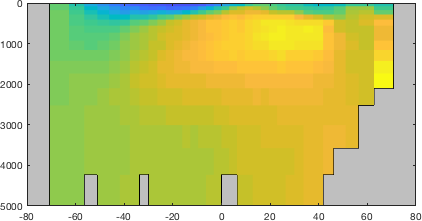
\includegraphics[width=0.95\linewidth]{../Separate_figures/BIOGEM/Atlantic_ocn_TDFe_profile.png}
 \label{fig:nutrients1}
\end{subfigure}%
\begin{subfigure}{.33\textwidth}
 \caption{Atlantic dFe - EcoGEnIE}
 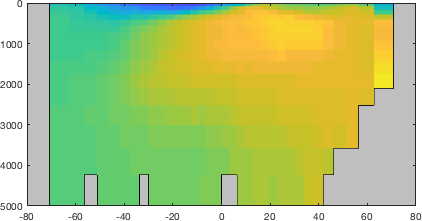
\includegraphics[width=0.95\linewidth]{../Separate_figures/ECOGEM/Atlantic_ocn_TDFe_profile.png}
 \label{fig:nutrients2}
\end{subfigure}
\begin{subfigure}{.33\textwidth}
 \caption{Indian dFe - cGEnIE}
 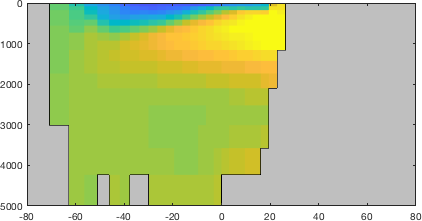
\includegraphics[width=0.95\linewidth]{../Separate_figures/BIOGEM/Indian_ocn_TDFe_profile.png}
 \label{fig:nutrients1}
\end{subfigure}%
\begin{subfigure}{.33\textwidth}
 \caption{Indian dFe - EcoGEnIE}
 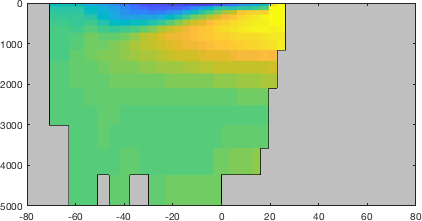
\includegraphics[width=0.95\linewidth]{../Separate_figures/ECOGEM/Indian_ocn_TDFe_profile.png}
 \label{fig:nutrients2}
\end{subfigure}
\begin{subfigure}{.33\textwidth}
 \caption{Pacific dFe - cGEnIE}
 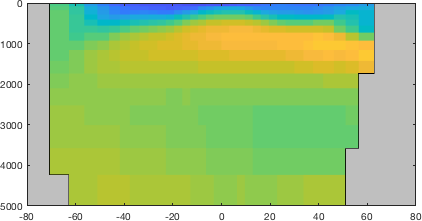
\includegraphics[width=0.95\linewidth]{../Separate_figures/BIOGEM/Pacific_ocn_TDFe_profile.png}
 \label{fig:nutrients1}
\end{subfigure}%
\begin{subfigure}{.33\textwidth}
 \caption{Pacific dFe - EcoGEnIE}
 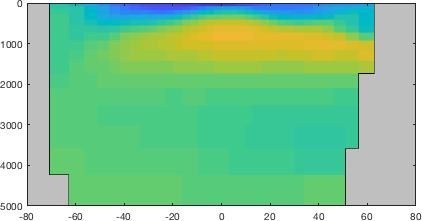
\includegraphics[width=0.95\linewidth]{../Separate_figures/ECOGEM/Pacific_ocn_TDFe_profile.png}
 \label{fig:nutrients2}
\end{subfigure}
\\[+0.2cm]
\begin{subfigure}{.5\textwidth}
 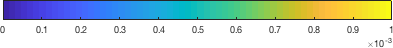
\includegraphics[width=0.95\linewidth]{../Separate_figures/ECOGEM/ocn_TDFe_profile_clrbr.png}
\end{subfigure}
\end{figure}



\end{document}